% ===================================================
% CHAPITRE 13 — AUTRES FAMILLES ANCIENNES
% Pages imprimées 67-71 — vues 70-74
% ===================================================
\chapter{Autres familles anciennes}

% --- Page imprimée 67 — vue 70
Armes des Testenoire de Beaujeu.
\begin{center}
    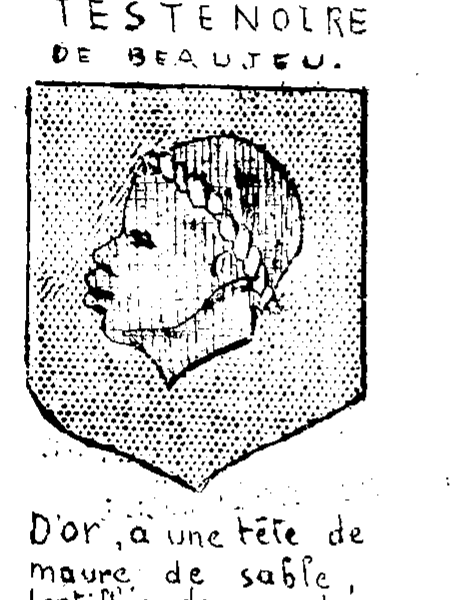
\includegraphics[width=0.22\textwidth]{Illustrations/illus-autres-testenoire.png}
\end{center}

Duligier - Testenoire

Le premier dont le nom nous est connu est Clément Ligier Testenoire qui vivait au début du XVIe siècle.

Jehan Testenoire dénommé Châtelain de la juridiction de Coux et Alloignet tomba malade, à Belleville dans la maison de Maître Anthoine Saulnay, chirurgien, et y mourut. Son testament porte la date du 28 Octobre 1586.

Pierre Testenoire, né en 1588 fut d'abord placé chez "Jéhan Barbier recteur des escolles de Beaujeu". Ce fut le premier qui prit le titre de notaire à Ouroux.

Jean Hugues Duligier Testenoire, né en 1625, succéda à son père comme notaire. Il prit une part active à toutes les affaires qui se traitèrent autour de lui. Commis greffier de la Vicomté du Thil, de la justice seigneuriale d'Arcis, d'Avenas, de Gorze, il rédigea un grand nombre d'actes de procédure qui existent encore dans les notariats de la contrée. Jusqu'à sa mort qui arriva en 1708 il seconda son fils Jean Chrysostome dans la gestion de ses biens. Par acte du 15 Juin 1707 il fonda, de concert avec lui, cinq Messes basses qui devaient être dites dans leur chapelle.

Jean Chrysostôme Duligier Testenoire, pour parer aux inconvénients résultant pour lui de la cote excessive que lui avaient imposée les habitants d'Ouroux, il se fit pourvoir de la charge de substitut du procureur du roi en l'élection de Beaujolais à cause du privilège accordé à cette charge de l'exemption des tailles et autres imposi
% --- Page imprimée 68 — vue 71 (suite)
tions. Marié en 1700 à Marie Anne Aulas, fille de Etienne Aulas notaire à St-Germain-la-Montagne, il mourut en 1729. Sa veuve échangea, en 1732, un bois de haute futaie chêne situé à Montchatail, de la semence de 45 mesures environ et estimé 5000 livres avec le domaine des Micoux, arrière fief situé à Vauxrenard.

Jean Chrysostôme Duligier eut dix enfants. Parmi ceux-ci signalons surtout Marie Françoise et Jean Marie.

Marie Françoise, baptisée le 2 Janvier 1709 eut pour parrain Mr Joseph Aulas chanoine d'Aigueperse. Entrée dans la communauté de la Visitation de Macon, elle dut, après la suppression des ordres monastiques, rentrer dans sa famille. Son neveu ne put qu'à grand peine obtenir pour elle la pension de 700 livres à laquelle elle avait droit en vertu de la même loi. Elle ne pouvait surtout obtenir un certificat de civisme et de non émigration. Voici le signalement, établi pour elle, à cet effet, à l'âge de 85 ans : "extrêmement courbée, 4 pieds 1/2, cheveux et sourcils blancs, yeux gris, nez un peu long visage rond, un peu ridé ; bouche ordinaire et menton rond". Elle mourut en Germinal an III à l'âge de 86 ans.

Jean Marie Duligier Testenoire, comme nous le font savoir ses livres de comptes était un homme d'une grande piété ; "J'ai fait semer écrit-il, dans mon domaine des Micouds, 4 mesures de froment lequel a bien pris en semence, grâce à Dieu et veuille nous bénir avec tous les fruits de la terre. Amen. Année 1766". "Le tout peut faire 12 chars de foin, encore bon foin, grâce à Dieu, quoiqu'il ait plu dessus, n'ayant pas eu grand mal parce qu'il était tout en (neaux ?)" Jean Marie mourut à l'âge de 71 ans. Il nous apprend lui-même qu'un de ses frères était notaire à Prissé.

Benoit Duligier Testenoire, fils du précédent résida à Ouroux, jusqu'en 1773, puis il s'installa comme notaire à Tramayes. En 1789 il revient à Ouroux remplacer Mr Pochon qui possédait le notariat, depuis 1750.

Benoit eut 5 enfants, mais avec l'un d'eux, Jean Antoine Marie qui mourut le 30 Novembre 1864, en revenant de Beaujeu, dans les bois d'Avenas, s'éteignit à Ouroux la branche aînée des Duligier-Testenoire.

Avant de terminer ce travail sur une des familles les plus im
% --- Page imprimée 69 — vue 72 (suite)
portantes de notre paroisse il est intéressant de rapporter les traditions généralement admises au sujet de l'origine du nom de Testenoire.

Mr Morétain et avec lui la France par cantons écrivent à ce sujet : "On raconte que le surnom de Testenoire leur vient d'une circonstance particulière. Jean de Bacot, d'une taille colossale, d'une force athlétique, gentilhomme de la maison du roi, se trouvait dans une bataille en 1572 où le roi assistait en personne. Le roi distinguant ce brave qui faisait des prodiges de valeur au milieu du combat (il était facile de le distinguer puisqu'il dépassait de toute la tête ses compagnons d'armes) demanda qu'elle était cette grande tête noire qu'il voyait comme un autre Mars exterminateur. On croit que c'est de ce mot que les Duligier ont pris le nom de Testenoire".

Remarquons que la date assignée plus haut est évidemment fautive, puisque le nom de Testenoire était donné aux Duligier dès 1520, comme nous le prouve le terrier d'Alloignet. Mais encore devons-nous accepter le fonds même de la tradition ? L'étude des documents nous permet de proposer une autre origine au nom qui nous occupe.

Dans une reconnaissance de servis faite en 1769 par Jean-Marie Duligier nous trouvons mentionnée une partie de jardin qui fut maison haute et basse, jadis appelée "la vieille teste noire" située au bourg d'Ouroux. Il s'agit ici du jardin appartenant aux MM Gonnet.

Reportons-nous aux détails donnés sur le fief de Naou et la destruction probable de son château vers la fin du XVIe siècle. Les débris de murailles calcinés et noircis par le feu se détachaient, comme des silhouettes sur l'horizon ; de là le nom de testes noires qui leur fut donné par les habitants du bourg. Plus tard ces restes de murailles disparurent, le sol conserva le nom de testes noires et les Duligier en étant devenus possesseurs, ajoutèrent ce surnom à leur nom primitif de Ligier. Au moyen âge le nom de la terre recouvrait souvent le nom de famille et le premier était seul en usage. C'est précisément ce qui eut lieu dans le cas qui nous occupe et cette hypothèse nous paraît la seule admissible.

% --- Page imprimée 70 — vue 73
De Fonte ou De La Font

Dans les titres anciens, cette famille porte le nom latin De Fonte qui plus tard fut traduit par De La Font.

Les membres de cette famille ont joué un rôle relativement important dans notre contrée par suite des charges qu'ils occupèrent dans le notariat aussi bien que dans les justices seigneuriales du Beaujolais. Au commencement du XVIIIe siècle, devenus fermiers pour la plupart, ils ne durent plus signer les actes dans lesquels ils figuraient comme contractants ou comme témoins. De là la transformation de leur nom en Laffont que Mr Costagne, curé, commença d'écrire en 1722 d'après la prononciation de l'époque; cette orthographe s'est conservée jusqu'à nos jours.

Le premier qui nous soit connu est N... De Fonte notaire à Ouroux en 1520. Il est probable que son père avait succédé à De Bosco vers le milieu du siècle précédent dans le notariat d'Ouroux.

Au début du XVIIe siècle, Antoine de la Font, vénérable et discrète personne était curé de Cenves. Son frère Thimothée lui avait donné une maison située au bourg d'Ouroux "sur la grande rue tenant du pont des Chasseignes à la croix du rempart d'Ouroux, près du colombier.

Thimothée de la Font gendarme de la compagnie du Duc de Nemours épouse Constance Bellon. Il céda à son fils tous ses biens. Son fils Ayné s'engagea à son tour à lui fournir "deux chambres garnies selon sa condition, savoir: d'un lit de plumes garni de coultres, coultrains et une couverture laine barriolée, quatre linceuils ràdeaux, autour a'icelluy, le tout thoile; deux plats, deux assiettes et deux écuelles, le tout étain; un pot de fer, une poëlle fer, une table avec ses tréteaux; un coffre pour mettre linge et pour la nourriture 24 mesures blé tendre, froment mesure de Beaujeu; une botte vin, 20 livres lard sallé et deux pintes huile".

Ayné de Lafont fils de Thimothée mourut en 1646. Marié à Suzanne Berthelon, celle-ci fit son testament en faveur de son mari résidant au lieu appelé "en chasteau Montaigne" actuellement au Berthu. Ils eurent 4 enfants dont Antoine qui épousa Catherine Alacoque cousine de la Bienheureuse Marguerite Marie. En 1675 il est qualifié de bourgeois d'Ouroux. Il n'eut pas d'enfants.

% --- Page imprimée 71 — vue 74
Famille Montel

Le nom des Montel paraît pour la première fois au milieu du XVIIe siècle, dans un acte par lequel ils reconnaissent l'honorabilité de Mr Chostard curé d'Ouroux. Ils sont fréquemment cités à cette époque comme leveurs de tailles, fermiers des dîmes et toujours nous les trouvons avec les membres de la famille Morin, marchands comme eux, en antagonisme avec les familles bourgeoises de la paroisse et spécialement avec les Duligier.

Voici les noms qui méritent d'être cités :

Jean, marié avec Antoinette Pichard dont nous parlerons à l'article concernant l'église d'Ouroux et les fondations qui eurent lieu.

Philibert, petit-fils de Jean, baptisé en 1676. Il eut pour parrain noble Philibert Bertet, escuier seigneur de Gorze et pour marraine : demoiselle Angèle ou Angélique Ausmonier, femme de Jean Chrysostôme Alacoque advocat au parlement et frère de la Bienheureuse.

Jean Claude, frère de Philibert, baptisé le 11 Juin 1682 eut pour parrain Jean Chrysostôme de Grosbois et pour marraine Claudine Alacoque dont nous n'avons pu déterminer la parenté avec la Bienheureuse.

\begin{center}
    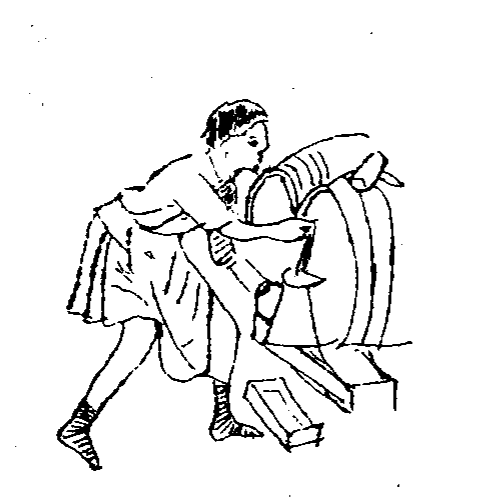
\includegraphics[width=0.28\textwidth]{Illustrations/illus-autres-scene-ouvrier.png}
    \hspace{0.04\textwidth}
    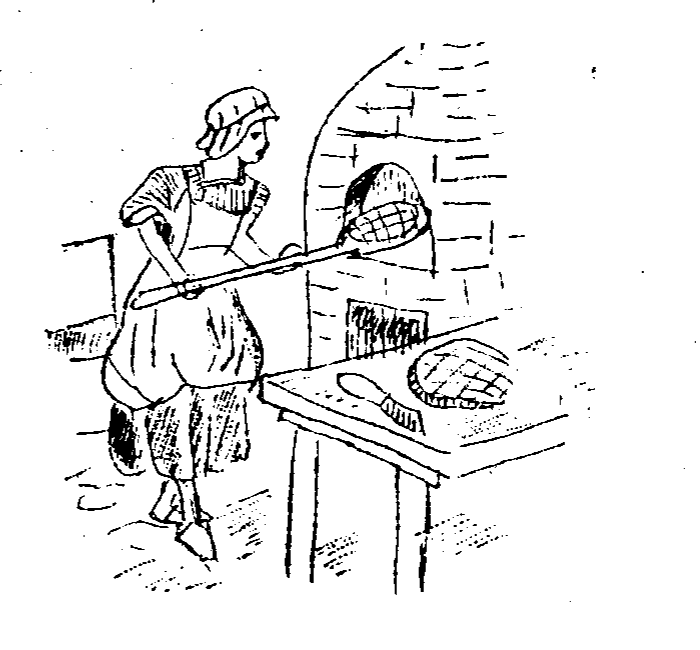
\includegraphics[width=0.34\textwidth]{Illustrations/illus-autres-scene-boulanger.png}
\end{center}
